\documentclass[11pt]{article}
\usepackage[paperwidth=8.5in, paperheight=11in]{geometry}
\usepackage{algorithm}
\usepackage{algorithmicx}
\usepackage[noend]{algpseudocode}
\usepackage{indentfirst}

\usepackage{tjimo}

\newcommand{\sevenpoints}{Time limit: 30 minutes.}
\newcommand{\righthead}{\fdbox{Round}{Practice Power}}

\usepackage{tikz}
\usepackage{amsmath}
\usepackage{amsthm}
\usepackage{amssymb}
%\usepackage{enumerate}
\usepackage{enumitem}
\usepackage{gensymb}
\usepackage{multicol}

\begin{comment}
\def \answer{\comment}
\def \solution{\comment}
\end{comment}

\begin{document}

\section{Introduction}

Unlike the other rounds, just getting the answer right is not enough on the Power Round. Make sure you explain your answer and use words to describe how you arrived at your answer. In the words of middle school math teachers across the nation -- no work, no credit!

This Practice Power Round (worth 25 points) is divided into two sections. In the first section,  we will discuss the shoelace theorem. We will then start proving the shoelace theorem for triangles.

Feel free to use results from previous problems (with the exception of using Section 1 for the other section) on this round and the practice power round to prove a problem (that is, you can use Problem 2 to prove Problem 3, but not vice versa). 

\section{The Shoelace Theorem}
\noindent The shoelace theorem can be used to calculate the area of polygons, given the Cartesian coordinates of the vertices. 

\begin{theorem}[The Shoelace Theorem] Suppose the polygon $P$ has vertices $(a_1, b_1)$, $(a_2, b_2)$, ... , $(a_n, b_n)$, listed in counterclockwise order. Then the area of $P$ is

\[\dfrac{1}{2} |(a_1b_2 + a_2b_3 + \cdots + a_nb_1) - (b_1a_2 + b_2a_3 + \cdots + b_na_1)|\]
\end{theorem}
\begin{comment}
The Shoelace Theorem gets its name because if one lists the coordinates in a column, 
\begin{align*} 
(a_1 &, b_1) \\ 
(a_2 &, b_2) \\ 
& \vdots \\ 
(a_n &, b_n) \\ 
(a_1 &, b_1) \\ 
\end{align*} 
and marks the pairs of coordinates to be multiplied, the resulting image looks like laced-up shoes.
\end{comment}

\begin{definition}
\[\left|\begin{array}{c c}a_1  & b_1 \\ a_2 &  b_2 \\ \vdots & \vdots \\ a_n & b_n \\ a_1 & b_1 \\ \end{array}\right| = \dfrac{1}{2} |(a_1b_2 + a_2b_3 + \cdots + a_nb_1) - (b_1a_2 + b_2a_3 + \cdots + b_na_1)|\]
Note that the shoelace theorem gets its name from the criss-crossing that results (in the first expression) when one marks the pairs of coordinates to be multiplied.
\end{definition}


\begin{problem}[2 points total]
Use shoelace to find, with proof, the area of the nonagon below:
\begin{center}
    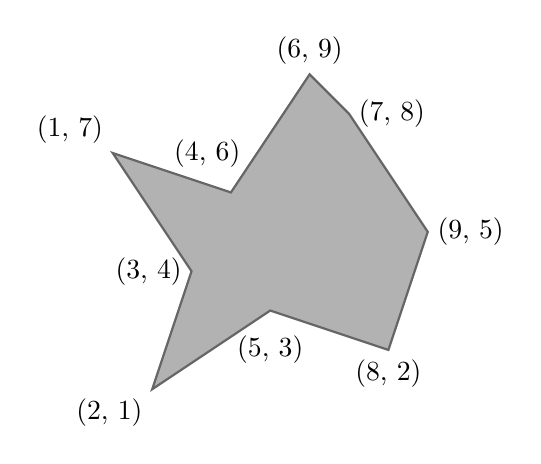
\begin{tikzpicture}
        \filldraw[color = black!60, fill = black!30, thick] (3, 4.5) -- (2, 3) -- (0.5, 3.5) -- (1.5, 2) -- (1, 0.5) -- (2.5, 1.5) -- (4, 1) -- (4.5, 2.5) -- (3.5, 4) -- cycle;
        \node at (3, 4.5) [above] {(6, 9)};
        \node at (1.7, 3.2) [above] {(4, 6)};
        \node at (0.5, 3.5) [above left] {(1, 7)};
        \node at (1.5, 2) [left] {(3, 4)};
        \node at (1, 0.5) [below left] {(2, 1)};
        \node at (2.5, 1.3) [below] {(5, 3)};
        \node at (4, 1) [below] {(8, 2)};
        \node at (4.5, 2.5) [right] {(9, 5)};
        \node at (3.5, 4) [right] {(7, 8)}; 
    \end{tikzpicture}
\end{center}
\end{problem}

\begin{answer} 41 \end{answer}
\begin{solution} Plugging the vertices into the shoelace theorem, we see that the area is 
\[\dfrac{1}{2} |(6)(6) + (4)(7) + (1)(4) + (3)(1) + (2)(3) + (5)(2) + (8)(5) + (9)(8) + (7)(9)\]
\[-((6)(8) + (4)(9) + (1)(6) + (3)(7) + (2)(4) + (5)(1) + (8)(3) + (9)(2) + (7)(2))|\]
\[=\frac{1}{2}(262-180)=\boxed{41}\]
\end{solution}

\begin{problem}[4 points total]
Prove that the shoelace theorem works for a triangle with a vertex at $(0, 0)$ and a base on the x-axis. (Hint: think of a way to describe the vertices.)
\end{problem}

\begin{solution}
Let the vertices be $(0, 0)$, $(x_2, 0)$, and $(x_1, y_1)$. Note that this works because one vertex is at the origin and the base is on the x-axis. The area of this triangle is $\frac{1}{2} bh = \frac{1}{2}|x_2y_1|$. Using shoelace, we see that the area is $\frac{1}{2}|(0)(0) + (x_2)(y_1) + (x_1)(0) - ((0)(x_2) + (0)(x_1) + (y_1)(0))| = \frac{1}{2}|x_2y_1|$. Since these two areas are equal, we are done.
\end{solution}

\begin{problem}[4 points total]
Prove that the shoelace theorem works for squares with one vertex on the x-axis and one vertex on the y-axis.
\end{problem}

\begin{solution}
Let the vertex on the x-axis be $(x, 0)$ and the vertex on the y-axis be $(0, y)$. Then, the remaining two vertices are at $(x+y, x)$ and $(y, x+y)$. The area of the square is $x^2+y^2$ by the Pythagorean theorem. Using shoelace, we get $\frac{1}{2}|(x)(y) + (0)(x+y) + (x)(y) + (x+y)(0)- ((0)(0) + (y)(y) + (x+y)(x+y) + (x)(x))| = \frac{1}{2}|xy+xy-y^2-x^2-2xy-y^2-x^2| = x^2+y^2$. Since these two areas are equal, we are done.
\end{solution}

\section{Areas of Triangles}

\noindent We will begin proving shoelace theorem for just triangles.
\subsection{Conveniently Located Triangles}
\noindent  Let the three vertices of triangle $ABC$ lie at $(0, 0), (x_1, y_1),$  and $(x_2, y_2)$.

\phantom{hello there}

\begin{problem}[5 points each]  Prove that the shoelace theorem applies to the following cases for $x_1, y_1, x_2, y_2 \geq 0$: (Hint: Draw a box around the triangle and subtract out unnecessary areas)
\end{problem}
\phantom{blahbity blah} 
\begin{multicols}{2}
\begin{enumerate}[label=(\alph*)]
\item $x_1 \leq x_2$ and $y_1 \geq y_2$
    \newline
    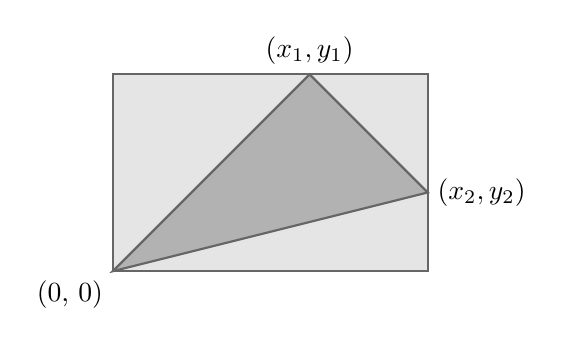
\begin{tikzpicture}
        \filldraw[color = black!60, fill = black!10, thick] (0, 0) -- (4, 0) -- (4, 2.5) -- (0, 2.5) -- cycle;
        \filldraw[color = black!60, fill = black!30, thick] (0, 0) -- (4, 1) -- (2.5, 2.5) -- cycle;
        \node at (0, 0) [below left] {(0, 0)};
        \node at (4, 1) [right] {$(x_2, y_2)$};
        \node at (2.5, 2.5) [above] {$(x_1, y_1)$};
    \end{tikzpicture}
\item $x_1 < x_2$ and $y_1 < y_2$
    \newline
    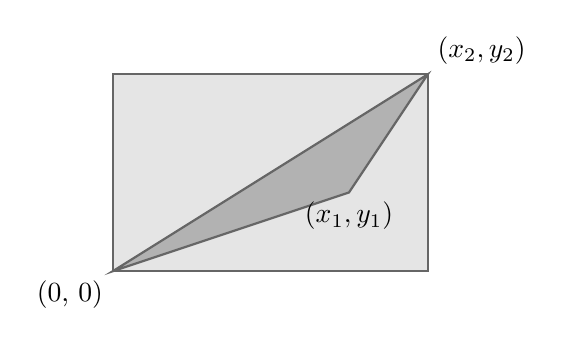
\begin{tikzpicture}
        \filldraw[color = black!60, fill = black!10, thick] (0, 0) -- (4, 0) -- (4, 2.5) -- (0, 2.5) -- cycle;
        \filldraw[color = black!60, fill = black!30, thick] (0, 0) -- (4, 2.5) -- (3, 1) -- cycle;
        \node at (0, 0) [below left] {(0, 0)};
        \node at (4, 2.5) [above right] {$(x_2, y_2)$};
        \node at (3, 1) [below] {$(x_1, y_1)$};
    \end{tikzpicture}
\end{enumerate}
\end{multicols}

\begin{solution}
\begin{enumerate}[label=(\alph*)]
\phantom{hello what's up}
\item The area is $x_2y_1 - (\frac{1}{2}x_1y_1+\frac{1}{2}x_2y_2+\frac{1}{2}(x_2-x_1)(y_1-y_2))$.
Expanding and cancelling gives $\frac{1}{2}(x_2y_1-x_1y_2)$. Note that this is the same result as when we use shoelace.

\item Note that there are two cases. 
\newline \textbf{Case 1:} $(x_2, y_2)$ is above the diagonal
The area is $x_1y_1 - (\frac{1}{2}(x_1-x_2)(y_1-y_2)+\frac{1}{2}x_2y_2+(x_2)(y_1-y_2)+\frac{1}{2}x_1y_1)$.
Expanding and cancelling gives $\frac{1}{2}(x_2y_1-x_1y_2)$. 
\newline \textbf{Case 2:} $(x_2, y_2)$ is below the diagonal
The area is $x_1y_1 - (\frac{1}{2}(x_1-x_2)(y_1-y_2)+\frac{1}{2}x_2y_2+(y_2)(x_1-x_2)+\frac{1}{2}x_1y_1)$.
Expanding and cancelling gives $\frac{1}{2}(x_2y_1-x_1y_2)$. 

\end{enumerate} \end{solution}

\subsection{General Triangles}

\begin{problem}[5 points total]  Prove that the shoelace theorem is consistent when a triangle is rotated by $90\degree$ counterclockwise about the origin. (Hint: $(x, y)$ becomes $(-y, x)$)
\end{problem}

\begin{solution}
The triangle with coordinates $(x_1, y_1), (x_2, y_2),$and $(x_3, y_3)$ becomes a triangle with coordinates $(-y_1, x_1), (-y_2, x_2),$and $(-y_3, x_3)$. Using shoelace on both yields $\frac{1}{2}|x_1y_2+x_2y_3+x_3y_1-y_1x_2-y_2x_3-y_3x_1|$ and $\frac{1}{2}|-y_1x_2-y_2x_3-y_3x_1+x_1y_2+x_2y_3+x_3y_1|$. Note that these two expressions are exactly the same. Thus, we are done.
\end{solution}

\begin{center}\textbf{*****PRACTICE POWER ENDS HERE. YOU HAVE BEEN WARNED.*****}\end{center}


\end{document}
